\documentclass[12pt,preprintnumbers,amsmath,amssymb,nofootinbib,superscriptaddress]{revtex4-1}
\usepackage[paperheight=12cm,top=0.5cm,bottom=0.5cm,left=1cm,right=1cm]{geometry}
\usepackage{xparse}
\NewDocumentCommand{\DIV}{om}{%
  \IfValueT{#1}{\setcounter{#2}{\numexpr#1-1\relax}}%
  \csname #2\endcsname
}

\usepackage{slashed}
\usepackage{amsmath}
\usepackage{textcomp}
\usepackage{amssymb}
\usepackage{amsfonts}
\usepackage{indentfirst}
\usepackage{color}
\usepackage[dvipsnames]{xcolor}
\usepackage{hyperref}
\usepackage{subcaption}
\usepackage{graphicx,graphics}
\graphicspath{{figures/}}
\usepackage[skins,theorems,many]{tcolorbox}
\tcbset{highlight math style={enhanced,
  colframe=red,colback=white,arc=0pt,boxrule=1pt}}
\usepackage[abs]{overpic}
\usepackage{xcolor,varwidth}
\usepackage[english]{babel}
\usepackage{blindtext,tikz}
\usetikzlibrary{calc,arrows.meta,positioning,decorations.pathreplacing}
\usepackage{fancyhdr}
\usepackage{enumitem}
\setlist[itemize]{nosep,leftmargin=1.2em,topsep=2pt,itemsep=2pt,before=\raggedright}
\hypersetup{colorlinks=true,citecolor=RoyalBlue,linkcolor=black,urlcolor=RoyalBlue}

\def\bibsection{\section*{}} %Removes black line above refrences

%--------------------------%
%----- COLOURED BOXES -----%
%--------------------------%

%Blue equation box
%\tcbhighmath[colframe=RoyalBlue!70!black,colback=RoyalBlue!25!white]{

%Orange equation box
%\tcbhighmath[colframe=BurntOrange!95!black,colback=BurntOrange!45!white]{

%Purple equation box
%\tcbhighmath[colframe=Purple!80!black,colback=Purple!30!white]{

%Green equation box
%\tcbhighmath[colframe=ForestGreen,colback=ForestGreen!25!white]{

%Grey equation box
%\tcbhighmath[colframe=Black,colback=Black!10!white]{

%Pink equation box
%\tcbhighmath[colframe=magenta,colback=magenta!20!white]{

%Blue and red equation box
%\tcbhighmath[frame style={left color=RoyalBlue!70!black,right color=Red!95!black},interior style={left color=RoyalBlue!35!white,right color=Red!50!white}]{

%Red and green equation box
%\tcbhighmath[frame style={left color=Red!95!black,right color=ForestGreen},interior style={left color=Red!50!white,right color=ForestGreen!25!white}]{

% Text boxes in the same colours as the equation boxes
\newtcolorbox{greybox}{colframe=Black,colback=Black!8!white,arc=0pt,boxrule=1pt,left=4pt,right=4pt,top=2pt,bottom=2pt}
\newtcolorbox{greenbox}{colframe=ForestGreen,colback=ForestGreen!15!white,arc=0pt,boxrule=1pt,left=4pt,right=4pt,top=2pt,bottom=2pt}
\newtcolorbox{bluebox}{colframe=RoyalBlue!70!black,colback=RoyalBlue!10!white,arc=0pt,boxrule=1pt,left=4pt,right=4pt,top=2pt,bottom=2pt}

% Footer line at the bottom of a slide
\newcommand{\slidefoot}[1]{\par\vspace{\fill}{\centering\footnotesize #1\par}}

% Diagram styles
\tikzset{
  box/.style={draw, rounded corners=2pt, align=center, inner sep=3pt, font=\small},
  cbox/.style={box, draw=RoyalBlue!70!black, fill=RoyalBlue!12},
  pbox/.style={box, draw=BurntOrange!95!black, fill=BurntOrange!18},
  gbox/.style={box, draw=ForestGreen, fill=ForestGreen!15},
  itemnode/.style={circle, draw=RoyalBlue!70!black, fill=RoyalBlue!15, minimum size=6.5mm, inner sep=0pt, font=\small},
  elemnode/.style={rectangle, draw=BurntOrange!95!black, fill=BurntOrange!20, minimum size=6mm, inner sep=0pt, font=\small},
  chosen/.style={fill=ForestGreen!35, draw=ForestGreen!70!black, very thick},
  arr/.style={-{Stealth[length=2.2mm]}, thick},
}

\begin{document}
\setlength{\parindent}{0pt}
\linespread{1}\selectfont % revtex preprint mode double-spaces text

\tikz[overlay,remember picture] % Side note
{
    \node at ($(current page.west)+(1,0)$) [rotate=90] {\Large\textcolor{gray}{SUKP -- work in progress}};
}

\pagenumbering{gobble}

\hfill{Research update -- October 2026} % Event and date

\vspace{2.5cm}

\title{
\tcbhighmath[frame style={left color=RoyalBlue!70!black,right color=Red!95!black},interior style={left color=RoyalBlue!35!white,right color=Red!50!white},boxrule=2pt]{
\text{\Large DQN-Guided E2LS for the Set-Union Knapsack Problem}
}}

\author{Your Name}

\affiliation{Your affiliation}


\maketitle

%==========================================================%
%  I. THE SET-UNION KNAPSACK PROBLEM  (1 slide)
%==========================================================%

\newpage

\DIV[1]{section}{The Set-Union Knapsack Problem}
\vspace{-0.35cm}
\DIV[1]{subsection}{Problem definition}
\vspace{-0.2cm}\hrule

\vspace{0.3cm}

\begin{minipage}[t]{0.56\textwidth}\vspace{0pt}
\small
\begin{itemize}
  \item $m$ items with profits $p_i$, $n$ elements with weights $w_j$, capacity $C$.
  \item Item $i$ covers a set of elements $U_i$. An element shared by several chosen items is paid \emph{once}.
\end{itemize}
\begin{equation*}
\tcbhighmath[colframe=Black,colback=Black!10!white]{
\max_{S}\ P(S)=\sum_{i\in S}p_i
\quad\text{s.t.}\quad
W(S)=\!\!\sum_{j\in\bigcup_{i\in S}U_i}\!\! w_j\le C}
\end{equation*}
\begin{itemize}
  \item NP-hard: the 0-1 knapsack problem is the case where no two items share an element~\cite{Goldschmidt1994,Arulselvan2014}.
  \item Benchmark: 60 instances. Set I: 30 with 85--500 items/elements~\cite{He2018}; Set II: 30 with 585--1000~\cite{Wei2021}.
  \item Density $\alpha\in\{0.10,0.15\}$ of the item-element relation; capacity $C=\beta\sum_j w_j$, $\beta\in\{0.75,0.85\}$.
\end{itemize}
\end{minipage}\hfill
\begin{minipage}[t]{0.40\textwidth}\vspace{0pt}
\centering
\vspace{0.4cm}
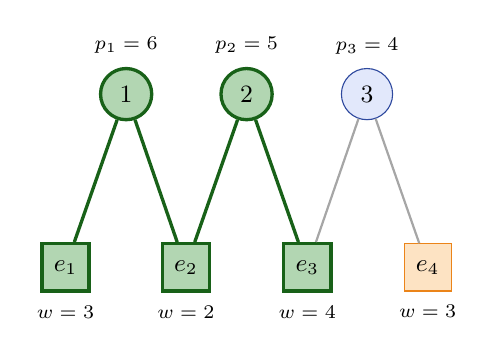
\begin{tikzpicture}[x=1.15cm,y=1cm]
  \node[itemnode,chosen] (i1) at (0.67,2.2) {$1$};
  \node[itemnode,chosen] (i2) at (2.00,2.2) {$2$};
  \node[itemnode]        (i3) at (3.33,2.2) {$3$};
  \node[above=0.5mm of i1, font=\scriptsize] {$p_1=6$};
  \node[above=0.5mm of i2, font=\scriptsize] {$p_2=5$};
  \node[above=0.5mm of i3, font=\scriptsize] {$p_3=4$};
  \node[elemnode,chosen] (e1) at (0.00,0) {$e_1$};
  \node[elemnode,chosen] (e2) at (1.33,0) {$e_2$};
  \node[elemnode,chosen] (e3) at (2.67,0) {$e_3$};
  \node[elemnode]        (e4) at (4.00,0) {$e_4$};
  \node[below=0.5mm of e1, font=\scriptsize] {$w=3$};
  \node[below=0.5mm of e2, font=\scriptsize] {$w=2$};
  \node[below=0.5mm of e3, font=\scriptsize] {$w=4$};
  \node[below=0.5mm of e4, font=\scriptsize] {$w=3$};
  \foreach \i/\j in {1/1,1/2,2/2,2/3} \draw[ForestGreen!70!black, very thick] (i\i) -- (e\j);
  \foreach \i/\j in {3/3,3/4} \draw[gray!70, thick] (i\i) -- (e\j);
\end{tikzpicture}

\vspace{0.2cm}
\footnotesize
$C=9$. Optimal $S=\{1,2\}$ covers $e_1,e_2,e_3$:\\
$W=3+2+4=9\le C$, $P=11$.\\
Paying per item would cost $5+6=11>C$.
\end{minipage}

%==========================================================%
%  II. OUR C++ SOLVER (E2LS)  (4 slides)
%==========================================================%

\newpage

\DIV[2]{section}{Our C++ solver (based on E2LS)}
\vspace{-0.35cm}
\DIV[1]{subsection}{Main loop}
\vspace{-0.2cm}\hrule

\vspace{0.5cm}

\begin{center}
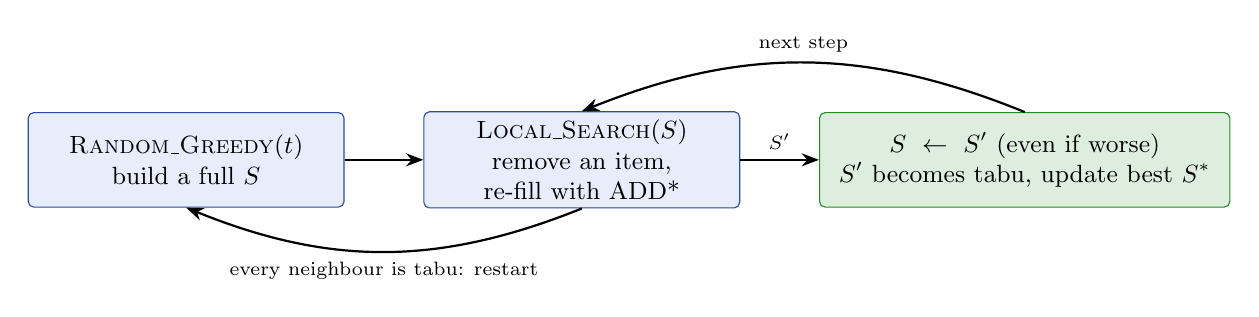
\begin{tikzpicture}[node distance=10mm]
  \node[cbox, text width=3.8cm, minimum height=12mm] (rg) {\textsc{Random\_Greedy}$(t)$\\ build a full $S$};
  \node[cbox, text width=3.8cm, minimum height=12mm, right=of rg] (ls) {\textsc{Local\_Search}$(S)$\\ remove an item, re-fill with ADD*};
  \node[gbox, text width=5.0cm, minimum height=12mm, right=of ls] (acc) {$S\leftarrow S'$ (even if worse)\\ $S'$ becomes tabu, update best $S^*$};
  \draw[arr] (rg) -- (ls);
  \draw[arr] (ls) -- node[above, font=\scriptsize]{$S'$} (acc);
  \draw[arr] (acc.north) to[bend right=22] node[above, font=\scriptsize]{next step} (ls.north);
  \draw[arr] (ls.south) to[bend left=22] node[below, font=\scriptsize]{every neighbour is tabu: restart} (rg.south);
\end{tikzpicture}
\end{center}

\vspace{0.2cm}
\small
\begin{minipage}[t]{0.49\textwidth}\vspace{0pt}
\begin{itemize}
  \item One step: try removing each of the $r_{num}$ lowest-ratio items, let ADD* re-fill the knapsack, keep the best non-tabu result $S'$.
  \item Move to $S'$ even when it is worse than $S$, to escape local optima.
\end{itemize}
\end{minipage}\hfill
\begin{minipage}[t]{0.49\textwidth}\vspace{0pt}
\begin{itemize}
  \item Tabu list: every accepted solution, stored as a 64-bit hash, so the search never cycles.
  \item Parameters as in the paper: $r_{num}=a_{num}=2$, $t=\sqrt{\max(m,n)}$. Stops on a time or step budget.
\end{itemize}
\end{minipage}

\slidefoot{\cite{Zhu2022} W. Zhu and L. Luo (2022)}

\newpage

\DIV[2]{section}{Our C++ solver (based on E2LS)}
\vspace{-0.35cm}
\DIV[2]{subsection}{Value-weight ratio and greedy construction}
\vspace{-0.2cm}\hrule

\vspace{0.3cm}

\begin{minipage}[t]{0.52\textwidth}\vspace{0pt}
\begin{equation*}
\tcbhighmath[colframe=RoyalBlue!70!black,colback=RoyalBlue!25!white]{
AW(S,i)=\sum_{j\in U_i,\ c_j=0} w_j,
\qquad
R(S,i)=\frac{p_i}{AW(S,i)}}
\end{equation*}
\small
\begin{itemize}
  \item $c_j$: number of chosen items covering element $j$.
  \item $AW$: weight that adding $i$ newly covers. For $i\in S$, the weight only $i$ covers ($c_j=1$).
  \item \emph{Free} items ($AW=0$) raise the profit at no cost: always added.
  \item High $R$: add or keep. Low $R$: remove first.
\end{itemize}
\end{minipage}\hfill
\begin{minipage}[t]{0.44\textwidth}\vspace{0pt}
\small
\begin{greybox}
\textbf{\textsc{Random\_Greedy}$(t)$}\\
repeat: add all free items;\\
\hspace*{1em}sample $t$ feasible candidates,\\
\hspace*{1em}add the one with the highest $R$\\
until no item fits
\end{greybox}
\vspace{0.2cm}
\begin{greenbox}
\textbf{Incremental state (C++)}\\
keep $c_j$ for every element: adding or removing item $i$ costs $O(|U_i|)$, and $W$ changes only when some $c_j$ goes $0\leftrightarrow 1$.
\end{greenbox}
\end{minipage}

\slidefoot{\cite{Zhu2022} W. Zhu and L. Luo (2022)}

\newpage

\DIV[2]{section}{Our C++ solver (based on E2LS)}
\vspace{-0.35cm}
\DIV[3]{subsection}{Local search and ADD*}
\vspace{-0.2cm}\hrule

\vspace{0.3cm}

\begin{minipage}[t]{0.56\textwidth}\vspace{0pt}
\centering
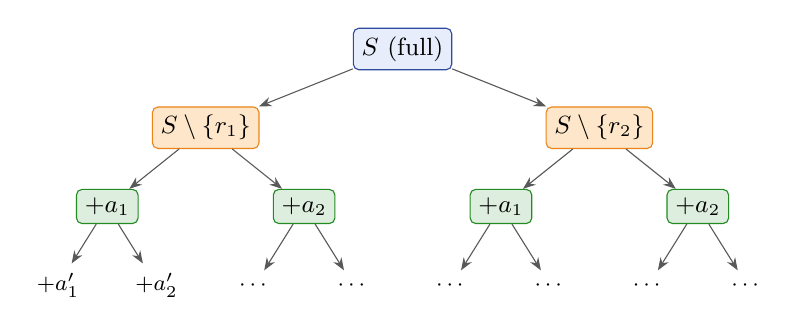
\begin{tikzpicture}[
  level distance=10mm,
  level 1/.style={sibling distance=50mm},
  level 2/.style={sibling distance=25mm},
  level 3/.style={sibling distance=12.5mm},
  every node/.style={font=\footnotesize},
  edge from parent/.style={draw, -{Stealth[length=1.6mm]}, gray!70!black}]
  \node[cbox] {$S$ (full)}
    child {node[pbox] {$S\setminus\{r_1\}$}
      child {node[gbox] {$+a_1$}
        child {node {$+a'_1$}}
        child {node {$+a'_2$}}}
      child {node[gbox] {$+a_2$}
        child {node {$\cdots$}}
        child {node {$\cdots$}}}}
    child {node[pbox] {$S\setminus\{r_2\}$}
      child {node[gbox] {$+a_1$}
        child {node {$\cdots$}}
        child {node {$\cdots$}}}
      child {node[gbox] {$+a_2$}
        child {node {$\cdots$}}
        child {node {$\cdots$}}}};
\end{tikzpicture}

\vspace{0.1cm}
{\scriptsize $r_1,r_2$: the two lowest-ratio items of $S$. $a_1,a_2$: the two best-ranked candidates at each node. A branch ends when nothing more fits.}
\end{minipage}\hfill
\begin{minipage}[t]{0.40\textwidth}\vspace{0pt}
\small
\begin{itemize}
  \item \textbf{Remove}: each of the $r_{num}=2$ lowest-$R$ items, one at a time.
  \item \textbf{ADD*}: add the free items, rank the feasible candidates $FC$, branch on the best $a_{num}=2$, recurse.
  \item Tabu solutions are skipped at every node.
  \item Result: the best non-tabu solution over both trees.
\end{itemize}
\vspace{0.2cm}
\begin{greenbox}
\textbf{Ranking $FC$ is where learning plugs in.}\\
Paper: by $R(S,i)$. Ours: by the DQN's $Q_\theta(s,\text{add } i)$ (Section III).
\end{greenbox}
\end{minipage}

\slidefoot{\cite{Zhu2022} W. Zhu and L. Luo (2022)}

\newpage

\DIV[2]{section}{Our C++ solver (based on E2LS)}
\vspace{-0.35cm}
\DIV[4]{subsection}{Implementation and Python binding}
\vspace{-0.2cm}\hrule

\vspace{0.4cm}

\begin{center}
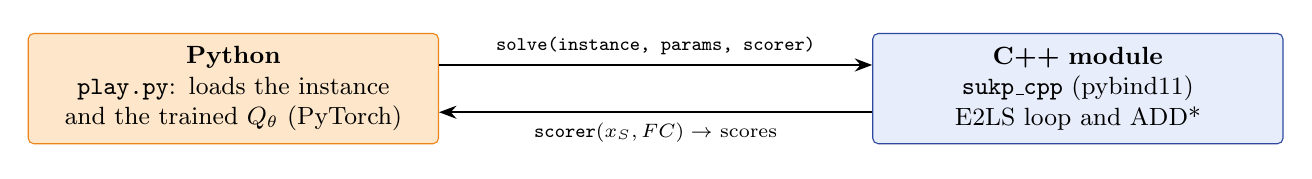
\begin{tikzpicture}
  \node[pbox, text width=5.0cm, minimum height=14mm] (py) {\textbf{Python}\\ \texttt{play.py}: loads the instance and the trained $Q_\theta$ (PyTorch)};
  \node[cbox, text width=5.0cm, minimum height=14mm, right=55mm of py] (cpp) {\textbf{C++ module} \texttt{sukp\_cpp} (pybind11)\\ E2LS loop and ADD*};
  \draw[arr] ([yshift=3mm]py.east) -- node[above, font=\scriptsize]{\texttt{solve(instance, params, scorer)}} ([yshift=3mm]cpp.west);
  \draw[arr] ([yshift=-3mm]cpp.west) -- node[below, font=\scriptsize]{\texttt{scorer}$(x_S, FC)\to$ scores} ([yshift=-3mm]py.east);
\end{tikzpicture}
\end{center}

\vspace{0.2cm}
\small
\begin{minipage}[t]{0.52\textwidth}\vspace{0pt}
\begin{itemize}
  \item C++17, \texttt{-O3}. The same search runs with the paper rule or with the network.
  \item The network is called only at ADD* nodes with more than $a_{num}$ candidates.
  \item Speed with the paper rule (one core): about 14{,}000 steps/s at $m=100$ and 240 steps/s at $m=1000$.
  \item Every returned solution is re-checked in Python.
\end{itemize}
\end{minipage}\hfill
\begin{minipage}[t]{0.44\textwidth}\vspace{0pt}
\begin{greybox}
\footnotesize
\begin{verbatim}
# ADD* as in the paper
python play.py --ranker ratio
# ADD* ranked by the pretrained DQN
python play.py --ranker dqn
\end{verbatim}
\end{greybox}
\end{minipage}

%==========================================================%
%  III. ADD* RANKED BY A PRETRAINED DQN  (5 slides)
%==========================================================%

\newpage

\DIV[3]{section}{ADD* ranked by a pretrained DQN}
\vspace{-0.35cm}
\DIV[1]{subsection}{Reinforcement learning in a nutshell}
\vspace{-0.2cm}\hrule

\vspace{0.3cm}

\begin{minipage}[t]{0.42\textwidth}\vspace{0pt}
\centering
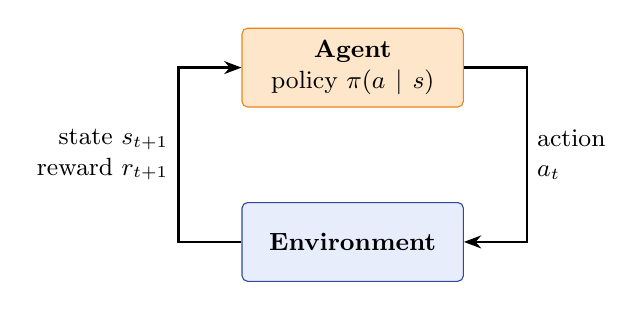
\begin{tikzpicture}
  \node[pbox, text width=2.6cm, minimum height=10mm] (agent) {\textbf{Agent}\\ policy $\pi(a\mid s)$};
  \node[cbox, text width=2.6cm, minimum height=10mm, below=12mm of agent] (env) {\textbf{Environment}};
  \draw[arr] (agent.east) -- ++(0.8,0) |- node[pos=0.25, right, font=\small, align=left]{action\\ $a_t$} (env.east);
  \draw[arr] (env.west) -- ++(-0.8,0) |- node[pos=0.25, left, font=\small, align=right]{state $s_{t+1}$\\ reward $r_{t+1}$} (agent.west);
\end{tikzpicture}

\vspace{0.3cm}
\begin{greenbox}
\small
\textbf{In our SUKP setting}\\
state $s$: the current solution $x_S$\\
action $a$: add or remove one item\\
reward $r$: gain in the best profit
\end{greenbox}
\end{minipage}\hfill
\begin{minipage}[t]{0.55\textwidth}\vspace{0pt}
\small
\begin{itemize}
  \item Goal: a policy that maximises the expected return $G_t=\sum_{k\ge 0}\gamma^k r_{t+k+1}$, with discount $\gamma\in[0,1)$.
  \item Action value $Q^\pi(s,a)=\mathbb{E}_\pi[\,G_t\mid s_t=s,\,a_t=a\,]$: how good action $a$ is in state $s$.
\end{itemize}
\begin{equation*}
\tcbhighmath[colframe=RoyalBlue!70!black,colback=RoyalBlue!25!white]{
Q^*(s,a)=\mathbb{E}\big[\,r+\gamma\max_{a'}Q^*(s',a')\,\big]}
\end{equation*}
\begin{itemize}
  \item Q-learning moves $Q(s,a)$ toward $r+\gamma\max_{a'}Q(s',a')$ after every step, then acts by $\arg\max_a Q(s,a)$.
  \item Exploration: $\varepsilon$-greedy tries a random action with probability $\varepsilon$.
  \item Too many states for a table ($2^m$ solutions), so $Q$ is approximated by a neural network: \textbf{DQN}.
\end{itemize}
\end{minipage}

\slidefoot{\cite{Sutton2018} R. S. Sutton and A. G. Barto (2018); \cite{Watkins1992} C. J. C. H. Watkins and P. Dayan (1992)}

\newpage

\DIV[3]{section}{ADD* ranked by a pretrained DQN}
\vspace{-0.35cm}
\DIV[2]{subsection}{Training first, then search}
\vspace{-0.2cm}\hrule

\vspace{0.4cm}

\begin{center}
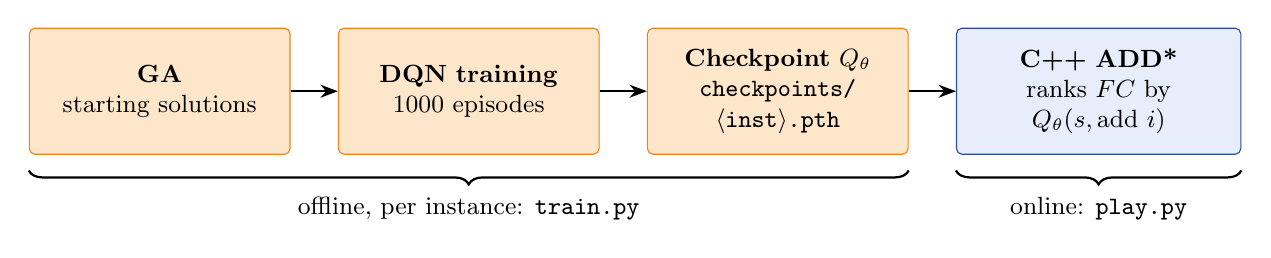
\begin{tikzpicture}[node distance=6mm]
  \node[pbox, text width=3.1cm, minimum height=16mm] (ga) {\textbf{GA}\\ starting solutions};
  \node[pbox, text width=3.1cm, minimum height=16mm, right=of ga] (dqn) {\textbf{DQN training}\\ 1000 episodes};
  \node[pbox, text width=3.1cm, minimum height=16mm, right=of dqn] (ck) {\textbf{Checkpoint} $Q_\theta$\\ \texttt{checkpoints/}\\ \texttt{$\langle$inst$\rangle$.pth}};
  \node[cbox, text width=3.4cm, minimum height=16mm, right=of ck] (add) {\textbf{C++ ADD*}\\ ranks $FC$ by $Q_\theta(s,\text{add } i)$};
  \draw[arr] (ga) -- (dqn);
  \draw[arr] (dqn) -- (ck);
  \draw[arr] (ck) -- (add);
  \draw[decorate, decoration={brace, mirror, amplitude=5pt}, thick]
    ([yshift=-2mm]ga.south west) -- node[below=6pt, font=\small]{offline, per instance: \texttt{train.py}} ([yshift=-2mm]ck.south east);
  \draw[decorate, decoration={brace, mirror, amplitude=5pt}, thick]
    ([yshift=-2mm]add.south west) -- node[below=6pt, font=\small]{online: \texttt{play.py}} ([yshift=-2mm]add.south east);
\end{tikzpicture}
\end{center}

\vspace{0.1cm}
\begin{minipage}[t]{0.50\textwidth}\vspace{0pt}
\small
\begin{itemize}
  \item \textbf{Training first}: on the instance, the DQN learns which single add/remove move improves a solution.
  \item \textbf{Then search}: E2LS runs unchanged except for how ADD* ranks its candidates.
  \item The gap input is set to $0$ at ADD* nodes, since ADD* only adds items.
\end{itemize}
\end{minipage}\hfill
\begin{minipage}[t]{0.47\textwidth}\vspace{0pt}
\begin{equation*}
\tcbhighmath[frame style={left color=RoyalBlue!70!black,right color=Red!95!black},interior style={left color=RoyalBlue!35!white,right color=Red!50!white}]{
\begin{aligned}
\text{paper:}\quad & \operatorname{rank}(i)=R(S,i)=p_i/AW(S,i)\\
\text{ours:}\quad & \operatorname{rank}(i)=Q_\theta\big((x_S,0),\ \text{add } i\big)
\end{aligned}}
\end{equation*}
\end{minipage}

\newpage

\DIV[3]{section}{ADD* ranked by a pretrained DQN}
\vspace{-0.35cm}
\DIV[3]{subsection}{GA generation of starting solutions}
\vspace{-0.2cm}\hrule

\vspace{0.3cm}

\begin{minipage}[t]{0.54\textwidth}\vspace{0pt}
\small
\begin{itemize}
  \item Binary GA (\texttt{mealpy}): population 50, 100 generations.
  \item Tournament selection ($k=10$), uniform crossover ($p_c=0.9$), bit-flip mutation ($p_m=0.4$).
  \item \textbf{Decoding}: add the items whose bit is 1 in index order, skipping any that would exceed $C$. Every individual is feasible and its fitness is $P(S)$.
  \item One GA run per episode gives 1000 good but different starting solutions.
\end{itemize}
\vspace{0.2cm}
\begin{greenbox}
\textbf{Why GA starts?} Episodes begin near good solutions, so the DQN learns the improving moves that matter where the search actually works.
\end{greenbox}
\end{minipage}\hfill
\begin{minipage}[t]{0.42\textwidth}\vspace{0pt}
\centering
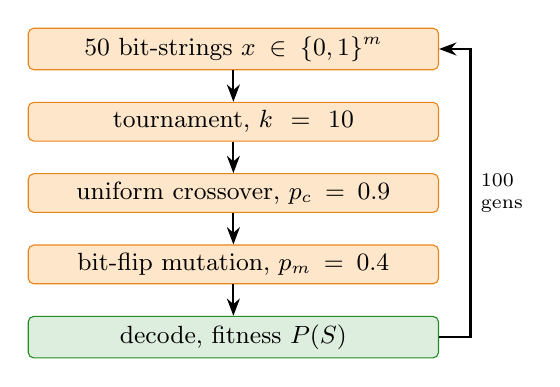
\begin{tikzpicture}[node distance=4mm]
  \node[pbox, text width=5.0cm] (pop) {50 bit-strings $x\in\{0,1\}^m$};
  \node[pbox, text width=5.0cm, below=of pop] (sel) {tournament, $k=10$};
  \node[pbox, text width=5.0cm, below=of sel] (cx) {uniform crossover, $p_c=0.9$};
  \node[pbox, text width=5.0cm, below=of cx] (mut) {bit-flip mutation, $p_m=0.4$};
  \node[gbox, text width=5.0cm, below=of mut] (ev) {decode, fitness $P(S)$};
  \draw[arr] (pop) -- (sel);
  \draw[arr] (sel) -- (cx);
  \draw[arr] (cx) -- (mut);
  \draw[arr] (mut) -- (ev);
  \draw[arr] (ev.east) -- ++(0.4,0) |- node[pos=0.25, right, font=\scriptsize, align=left]{100\\ gens} (pop.east);
\end{tikzpicture}
\end{minipage}

\newpage

\DIV[3]{section}{ADD* ranked by a pretrained DQN}
\vspace{-0.35cm}
\DIV[4]{subsection}{DQN: state, actions, reward, training}
\vspace{-0.2cm}\hrule

\vspace{0.3cm}

\begin{minipage}[t]{0.50\textwidth}\vspace{0pt}
\small
\begin{itemize}
  \item \textbf{State} $s=(x_S,g)$: $x_S\in\{0,1\}^m$ marks the chosen items, $g=(P_{best}-P(S))/\bar p$ is the gap to the episode's best ($\bar p$: mean item profit).
  \item \textbf{Actions}: add $i$ or remove $i$ ($2m$ outputs). Infeasible moves are masked; undoing a recent move is tabu for 30 steps.
  \item \textbf{Reward}: only new bests count,
  $r_t=\max\big(0,\,P(S_{t+1})-P_{best}\big)/\bar p$,
  so an episode's return equals its total improvement of the best.
\end{itemize}
\end{minipage}\hfill
\begin{minipage}[t]{0.46\textwidth}\vspace{0pt}
\begin{equation*}
\tcbhighmath[colframe=Purple!80!black,colback=Purple!30!white]{
\begin{aligned}
y&=r+\gamma\max_{a'\in\mathcal{A}(s')}Q_{\bar\theta}(s',a')\\
\mathcal{L}(\theta)&=\big(Q_\theta(s,a)-y\big)^2
\end{aligned}}
\end{equation*}
\small
\begin{itemize}
  \item 1000 episodes of 100 steps; replay buffer $10^4$, batch 128.
  \item Target network $Q_{\bar\theta}$ synced every 5 episodes; $\gamma=0.99$; Adam, learning rate $10^{-3}$.
  \item Exploration: $\varepsilon$-greedy ($\varepsilon_0=1$, $\times 0.99$ per episode), otherwise sample from $\mathrm{softmax}(Q/\tau)$, $\tau=5$.
\end{itemize}
\end{minipage}

\slidefoot{\cite{Mnih2015} V. Mnih \textit{et al.} (2015)}

\newpage

\DIV[3]{section}{ADD* ranked by a pretrained DQN}
\vspace{-0.35cm}
\DIV[5]{subsection}{Graph neural network: message passing}
\vspace{-0.2cm}\hrule

\vspace{0.3cm}

\begin{minipage}[t]{0.38\textwidth}\vspace{0pt}
\centering
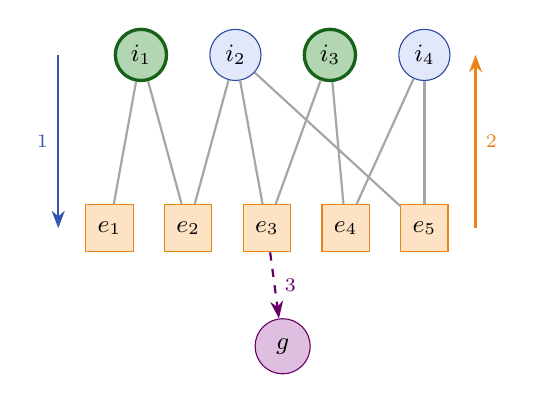
\begin{tikzpicture}[x=1cm,y=1cm]
  \node[itemnode,chosen] (I1) at (0.6,2.8) {$i_1$};
  \node[itemnode]        (I2) at (1.8,2.8) {$i_2$};
  \node[itemnode,chosen] (I3) at (3.0,2.8) {$i_3$};
  \node[itemnode]        (I4) at (4.2,2.8) {$i_4$};
  \foreach \k/\x in {1/0.2,2/1.2,3/2.2,4/3.2,5/4.2} \node[elemnode] (E\k) at (\x,0.6) {$e_\k$};
  \foreach \i/\j in {1/1,1/2,2/2,2/3,3/3,3/4,4/4,4/5,2/5} \draw[gray!70, thick] (I\i) -- (E\j);
  \node[circle, draw=Purple!80!black, fill=Purple!25, minimum size=7mm, font=\small] (G) at (2.4,-0.9) {$g$};
  \draw[arr, RoyalBlue!80!black] (-0.45,2.8) -- node[left, font=\scriptsize]{1} (-0.45,0.6);
  \draw[arr, BurntOrange!95!black] (4.85,0.6) -- node[right, font=\scriptsize]{2} (4.85,2.8);
  \draw[arr, Purple!80!black, dashed] (E3) -- node[right, font=\scriptsize]{3} (G);
\end{tikzpicture}

\vspace{0.1cm}
{\scriptsize Items (circles, green = chosen), elements (squares), global node $g$. One round: (1) items to elements, (2) elements to items, (3) readout to $g$.}
\end{minipage}\hfill
\begin{minipage}[t]{0.59\textwidth}\vspace{0pt}
\small
Inputs: items $h^I_i$ (chosen, profit, $AW$ to add / remove, fits, efficiency), elements $h^E_j$ (weight, covered, covered once, $c_j/\deg j$), global $g$ ($W/C$, residual capacity, gap, $|S|/m$). Then three rounds of
\begin{equation*}
\tcbhighmath[colframe=Black,colback=Black!10!white]{
\begin{aligned}
h^E_j &\leftarrow \mathrm{LN}\big(h^E_j+\phi_E[\,h^E_j,\ \operatorname{mean}_{i\ni j}h^I_i,\ \operatorname{mean}_{i\in S,\,i\ni j}h^I_i\,]\big)\\
h^I_i &\leftarrow \mathrm{LN}\big(h^I_i+\phi_I[\,h^I_i,\ \operatorname{mean}_{j\in U_i}h^E_j,\ g\,]\big)\\
g &\leftarrow \mathrm{LN}\big(g+\phi_G[\,g,\ \operatorname{mean}_i h^I_i,\ \operatorname{mean}_j h^E_j\,]\big)
\end{aligned}}
\end{equation*}
Heads shared by all items: $Q(s,\text{add } i)=\psi_{add}[h^I_i,g]$, $Q(s,\text{remove } i)=\psi_{rem}[h^I_i,g]$, so the number of parameters does not depend on $m$ or $n$.
\end{minipage}

\slidefoot{\cite{Gilmer2017} J. Gilmer \textit{et al.} (2017)}

%==========================================================%
%  IV. RESULTS  (3 slides)
%==========================================================%
% TODO: "Ours" is results_csv/profit.csv (30 s, seed 1), produced before the solver followed the
% paper's acceptance rule; rerun with the current solver before presenting final numbers.
% The profit tables below are generated from that CSV; regenerate them after the rerun.

\newpage

\DIV[4]{section}{Results}
\vspace{-0.35cm}
\DIV[1]{subsection}{Profit per instance: Set I}
\vspace{-0.2cm}\hrule

\vspace{0.3cm}

{\centering\scriptsize\setlength{\tabcolsep}{4pt}
\begin{tabular}{lrrrrrr}
\hline\hline
\multicolumn{7}{c}{$\alpha=0.10,\ \beta=0.75$}\\
\hline
$m\times n$ & BABC & QL & gbPSO & Best$^{\dagger}$ & \textbf{Ours} & $\Delta$\\
\hline
85$\times$100 & 11664 & 11619 & \textbf{12045} & \textbf{12045} & \textbf{12045} & 0\\
100$\times$85 & 13251 & 13251 & \textbf{13283} & \textbf{13283} & \textbf{13283} & 0\\
100$\times$100 & 13860 & \textbf{14044} & \textbf{14044} & \textbf{14044} & \textbf{14044} & 0\\
185$\times$200 & 13047 & 13503 & \textbf{13696} & \textbf{13696} & \textbf{13696} & 0\\
200$\times$185 & 13241 & 13405 & 13405 & \textbf{13521} & \textbf{13521} & 0\\
200$\times$200 & 11846 & 12196 & \textbf{12522} & \textbf{12522} & \textbf{12522} & 0\\
285$\times$300 & 11158 & 11395 & \textbf{11568} & \textbf{11568} & \textbf{11568} & 0\\
300$\times$285 & 10428 & 10952 & 11335 & \textbf{11563} & \textbf{11563} & 0\\
300$\times$300 & 12186 & 12644 & 12695 & \textbf{12817} & \textcolor{Red!80!black}{12784} & $-33$\\
385$\times$400 & 10085 & 10022 & 10483 & \textbf{10600} & \textcolor{Red!80!black}{10490} & $-110$\\
400$\times$385 & 10766 & 11242 & \textbf{11484} & \textbf{11484} & \textbf{11484} & 0\\
400$\times$400 & 10626 & 11158 & 11432 & \textbf{11665} & \textbf{11665} & 0\\
485$\times$500 & 10823 & 10823 & 11097 & \textbf{11321} & \textcolor{Red!80!black}{11119} & $-202$\\
500$\times$485 & 10784 & 11414 & \textbf{11771} & \textbf{11771} & \textcolor{Red!80!black}{11722} & $-49$\\
500$\times$500 & 10755 & 10888 & 10991 & \textbf{11249} & \textcolor{Red!80!black}{11245} & $-4$\\
\hline\hline
\end{tabular}
\hfill
\begin{tabular}{lrrrrrr}
\hline\hline
\multicolumn{7}{c}{$\alpha=0.15,\ \beta=0.85$}\\
\hline
$m\times n$ & BABC & QL & gbPSO & Best$^{\dagger}$ & \textbf{Ours} & $\Delta$\\
\hline
85$\times$100 & \textbf{12369} & \textbf{12369} & \textbf{12369} & \textbf{12369} & \textbf{12369} & 0\\
100$\times$85 & 12238 & \textbf{12479} & 12348 & \textbf{12479} & \textbf{12479} & 0\\
100$\times$100 & \textbf{13508} & \textbf{13508} & \textbf{13508} & \textbf{13508} & \textbf{13508} & 0\\
185$\times$200 & 10602 & 10973 & \textbf{11298} & \textbf{11298} & \textbf{11298} & 0\\
200$\times$185 & 13829 & 14044 & \textbf{14215} & \textbf{14215} & \textbf{14215} & 0\\
200$\times$200 & 11521 & 11911 & \textbf{12317} & \textbf{12317} & \textcolor{Red!80!black}{12113} & $-204$\\
285$\times$300 & 10528 & 11377 & 11763 & \textbf{11802} & \textcolor{Red!80!black}{11714} & $-88$\\
300$\times$285 & 12012 & 12245 & 12245 & \textbf{12607} & \textcolor{Red!80!black}{12500} & $-107$\\
300$\times$300 & 10382 & 11282 & 11425 & \textbf{11585} & \textbf{11585} & 0\\
385$\times$400 & 9456 & 9738 & 10302 & \textbf{10506} & \textcolor{Red!80!black}{10490} & $-16$\\
400$\times$385 & 9649 & 10419 & 10526 & \textbf{11209} & \textcolor{Red!80!black}{10758} & $-451$\\
400$\times$400 & 9541 & 10520 & 10927 & \textbf{11325} & \textbf{11325} & 0\\
485$\times$500 & 9333 & 9649 & 10117 & \textbf{10220} & \textcolor{Red!80!black}{10120} & $-100$\\
500$\times$485 & 9090 & 9729 & 10022 & \textbf{10238} & \textcolor{Red!80!black}{9938} & $-300$\\
500$\times$500 & 9318 & 9938 & 10194 & \textbf{10381} & \textcolor{Red!80!black}{10186} & $-195$\\
\hline\hline
\end{tabular}
\par}

\vspace{0.2cm}
{\footnotesize $^{\dagger}$I2PLS, KBTS, E2LS and AES-BM all reach this value on every Set I instance. Bold: best value in the row. $\Delta$ = Ours $-$ best. Ours reaches the best value on 17/30 instances.\par}

\slidefoot{Data: \texttt{results\_csv/profit.csv}. BABC~\cite{He2018}, QL and gbPSO~\cite{Ozsoydan2023}, I2PLS~\cite{Wei2019}, KBTS~\cite{Wei2021}, E2LS~\cite{Zhu2022}, AES-BM~\cite{Zhao2024}}

\newpage

\DIV[4]{section}{Results}
\vspace{-0.35cm}
\DIV[2]{subsection}{Profit per instance: Set II}
\vspace{-0.2cm}\hrule

\vspace{0.3cm}

{\centering\scriptsize\setlength{\tabcolsep}{4pt}
\begin{tabular}{lrrrr}
\hline\hline
\multicolumn{5}{c}{$\alpha=0.10,\ \beta=0.75$}\\
\hline
$m\times n$ & KBTS & E2LS & \textbf{Ours} & $\Delta$\\
\hline
585$\times$600 & \textbf{10393} & \textbf{10393} & \textcolor{Red!80!black}{10198} & $-195$\\
600$\times$585 & \textbf{9914} & \textbf{9914} & \textcolor{Red!80!black}{9688} & $-226$\\
600$\times$600 & \textbf{10524} & \textbf{10524} & \textcolor{Red!80!black}{10391} & $-133$\\
685$\times$700 & \textbf{10121} & \textbf{10121} & \textcolor{Red!80!black}{10103} & $-18$\\
700$\times$685 & \textbf{9881} & \textbf{9881} & \textcolor{Red!80!black}{9781} & $-100$\\
700$\times$700 & \textbf{9786} & \textbf{9786} & \textcolor{Red!80!black}{9709} & $-77$\\
785$\times$800 & \textbf{9384} & \textbf{9384} & \textcolor{Red!80!black}{9192} & $-192$\\
800$\times$785 & 9837 & \textbf{9937} & \textcolor{Red!80!black}{9698} & $-239$\\
800$\times$800 & \textbf{9932} & \textbf{9932} & \textcolor{Red!80!black}{9787} & $-145$\\
885$\times$900 & \textbf{9318} & \textbf{9318} & \textbf{9318} & 0\\
900$\times$885 & \textbf{9725} & \textbf{9725} & \textcolor{Red!80!black}{9594} & $-131$\\
900$\times$900 & \textbf{9745} & \textbf{9745} & \textcolor{Red!80!black}{9648} & $-97$\\
985$\times$1000 & 9193 & \textbf{9234} & \textcolor{Red!80!black}{9101} & $-133$\\
1000$\times$985 & 9668 & \textbf{9689} & \textbf{9689} & 0\\
1000$\times$1000 & 9544 & \textbf{9551} & \textcolor{Red!80!black}{9433} & $-118$\\
\hline\hline
\end{tabular}
\hfill
\begin{tabular}{lrrrr}
\hline\hline
\multicolumn{5}{c}{$\alpha=0.15,\ \beta=0.85$}\\
\hline
$m\times n$ & KBTS & E2LS & \textbf{Ours} & $\Delta$\\
\hline
585$\times$600 & \textbf{9256} & \textbf{9256} & \textcolor{Red!80!black}{9119} & $-137$\\
600$\times$585 & \textbf{9357} & \textbf{9357} & \textcolor{Red!80!black}{9252} & $-105$\\
600$\times$600 & \textbf{9062} & \textbf{9062} & \textcolor{Red!80!black}{8893} & $-169$\\
685$\times$700 & \textbf{9176} & \textbf{9176} & \textcolor{Red!80!black}{9064} & $-112$\\
700$\times$685 & \textbf{9163} & \textbf{9163} & \textcolor{Red!80!black}{9051} & $-112$\\
700$\times$700 & \textbf{9229} & \textbf{9229} & \textcolor{Red!80!black}{9154} & $-75$\\
785$\times$800 & \textbf{8746} & \textbf{8746} & \textcolor{Red!80!black}{8505} & $-241$\\
800$\times$785 & \textbf{9024} & \textbf{9024} & \textcolor{Red!80!black}{8898} & $-126$\\
800$\times$800 & \textbf{9101} & \textbf{9101} & \textcolor{Red!80!black}{8831} & $-270$\\
885$\times$900 & \textbf{8425} & \textbf{8425} & \textbf{8425} & 0\\
900$\times$885 & \textbf{8620} & \textbf{8620} & \textcolor{Red!80!black}{8342} & $-278$\\
900$\times$900 & \textbf{8990} & \textbf{8990} & \textcolor{Red!80!black}{8965} & $-25$\\
985$\times$1000 & 8528 & \textbf{8612} & \textcolor{Red!80!black}{8426} & $-186$\\
1000$\times$985 & 8453 & \textbf{8455} & \textcolor{Red!80!black}{8344} & $-111$\\
1000$\times$1000 & 8474 & \textbf{8538} & \textcolor{Red!80!black}{8248} & $-290$\\
\hline\hline
\end{tabular}
\par}

\vspace{0.2cm}
{\footnotesize Only KBTS and E2LS report Set II results. Bold: best value in the row. $\Delta$ = Ours $-$ best. Ours reaches the best value on 3/30 instances and is 18--290 below it on the others.\par}

\slidefoot{Data: \texttt{results\_csv/profit.csv}. KBTS~\cite{Wei2021}, E2LS~\cite{Zhu2022}}

\newpage

\DIV[4]{section}{Results}
\vspace{-0.35cm}
\DIV[3]{subsection}{Summary on the 60 benchmark instances}
\vspace{-0.2cm}\hrule

\vspace{0.3cm}

\begin{minipage}[t]{0.56\textwidth}\vspace{0pt}
\centering
\small
\begin{tabular}{lcccc}
\hline\hline
 & \multicolumn{2}{c}{Set I (30)} & \multicolumn{2}{c}{Set II (30)}\\
\cline{2-3}\cline{4-5}
Method & \#best & gap (\%) & \#best & gap (\%)\\
\hline
BABC~\cite{He2018}       & 2  & 6.18 & -- & --\\
I2PLS~\cite{Wei2019}     & 30 & 0.00 & -- & --\\
KBTS~\cite{Wei2021}      & 30 & 0.00 & 23 & 0.12\\
E2LS~\cite{Zhu2022}      & 30 & 0.00 & 30 & 0.00\\
QL~\cite{Ozsoydan2023}   & 4  & 3.07 & -- & --\\
gbPSO~\cite{Ozsoydan2023} & 13 & 1.11 & -- & --\\
AES-BM~\cite{Zhao2024}   & 30 & 0.00 & -- & --\\
\hline
\textbf{Ours} (C++ solver) & 17 & 0.56 & 3 & 1.45\\
\hline\hline
\end{tabular}
\end{minipage}\hfill
\begin{minipage}[t]{0.41\textwidth}\vspace{0pt}
\small
\begin{itemize}
  \item \#best: instances where the method reaches the best value in the table. Gap: mean of $(P_{best}-P)/P_{best}$.
  \item Ours is better than BABC on 28/30 and QL on 26/30 instances; against gbPSO: 14 better, 11 equal, 5 worse.
  \item Ours: one 30\,s run with the paper's ADD* ranking. E2LS: best of 10 runs, 500\,s (Set I) / 1000\,s (Set II).
  \item DQN-ranked ADD*: training in progress.
\end{itemize}
\end{minipage}

\slidefoot{Data: \texttt{results\_csv/profit.csv}}

%==========================================================%

\newpage

\DIV[5]{section}{References}
\vspace{-0.2cm}\hrule

{\providecommand{\bibfont}{}\renewcommand{\bibfont}{\scriptsize}\setlength{\bibsep}{1pt}
\bibliographystyle{unsrt}
\bibliography{Bibliography}
}

\vspace{\fill}
{\centering
\href{https://www.overleaf.com/latex/templates/academic-presentation-template/jpgfpsstrwzd}{Template submitted by D. Backhouse}\par}

\end{document}
